\chapter{The experiment}


The key feature of the experiment is the possibility to prepare few atoms in a microscopic dipole trap with high fidelity. For this, we have to prepare a degenerate quantum gas of fermionic Lithium-6 atoms. A brief summary of our apparatus and the preparation scheme is given in this chapter. A more detailed description can be found in \cite{friedhelm}. 

\section{Preparing a Fermi gas}
After vaporizing Lithium in an oven at 356 °C, the first component of the experiment is the Zeeman slower, that slows down the atomic beam with a resonant counterpropagating laser beam before it can be trapped inside the \textsc{mot}. The slower is essentially a large tube behind the oven shutter (see figure \ref{experiment}), surrounded by coils. A strong laser beam is pointing along the slower in the opposite direction of the flying atoms. When being in resonance with an atomic transition, the photons get absorbed and the atoms are pushed in the direction of the laser. Because spontaneous emission is directed in random directions, this leads to slowing of the cloud. During their deceleration, the transition frequency of the atoms is Doppler-shifted with respect to the laser beam. Therefore a spatially varying magnetic field shifts the atoms back into resonance by use of the Zeeman effect. 
\begin{figure}[h]
\centering
\begin{subfigure}[b]{0.8\textwidth}
                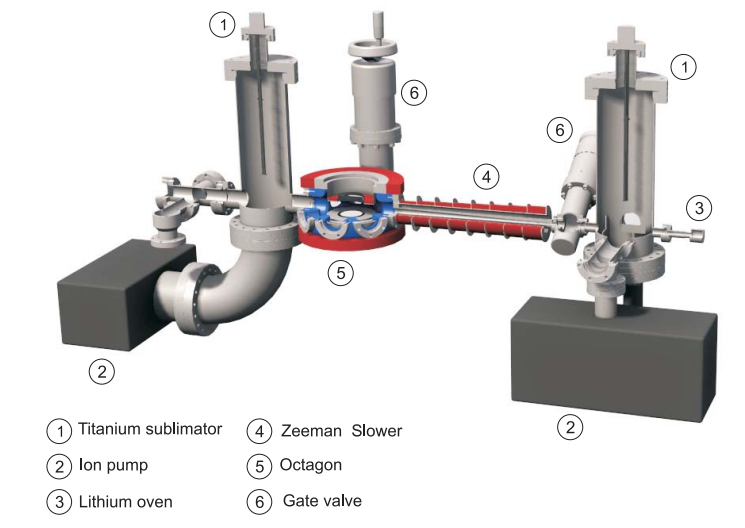
\includegraphics[width=\textwidth]{exsetup}
\end{subfigure}
\caption{Model of the experiments core-components. On the left the octagon-shaped vacuum chamber is visible, in which the experiment is carried out. Trough the view ports lasers for the \textsc{mot} and dipole-trap enter the chamber, (see figure \ref{scheme}). It is surrounded by coils providing magnetic field for several stages of the process. On the right one can see the oven and the Zeeman-slower connecting both parts.}
\label{experiment}
\end{figure}

After leaving the Zeeman slower, the atoms are captured in a magneto-optical trap (\textsc{mot})
It consists of six counter-propagating near-resonant laser beams. The usage of many retro-reflected beams in different directions makes it possible not only to force the atoms in a certain direction, but to also affect all particles with a high absolute velocity. This reduces the overall average-speed and therefore cools the gas. However, since the force of the laser beams alone is only velocity-dependent, slow particles would exit the center of the crossed beams over time. For this reason a magneto-optical trap uses a magnetic quadrupole-field, that has zero strength in the middle and increases when moving further away from the center. The Zeeman-effect shifts the level-distance for the out moving atoms towards the frequency of the laser, which will then apply a force, dependent on the spatial position, enabling not only cooling but trapping and compression of the gas-sample. The natural linewidth of the used transition limits the cooling of the \textsc{mot} to a temperature of around 140$\mu \mathrm{K}$. The system used in this experiment can store around 10⁸ atoms. 

However, to obtain a degenerate Fermi gas, the temperature has to be reduced much further. The next step on this ladder is to transfer the atoms from the \textsc{mot} into the crossed dipole trap. 
%\begin{figure}[h]
%\centering
%\begin{subfigure}[b]{0.8\textwidth}
%                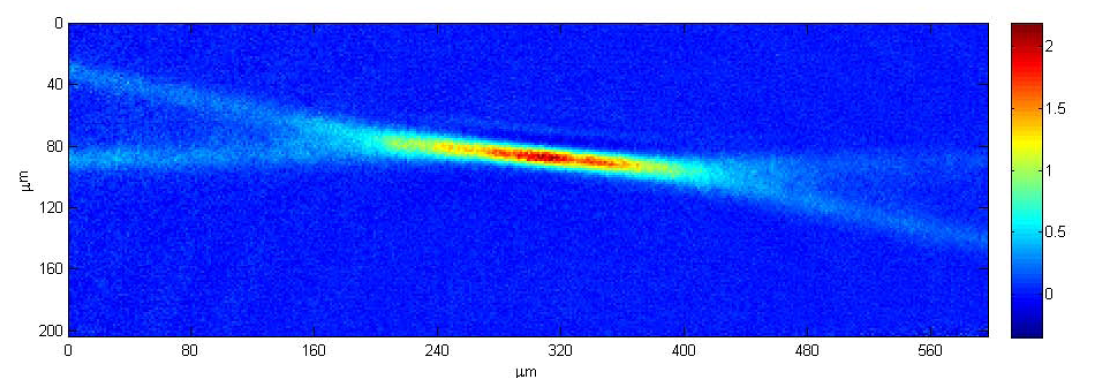
\includegraphics[width=\textwidth]{dipolefoto}
%\end{subfigure}
%\caption{Absorbtion image of the crossed dipole trap \cite{lompe}.}
%\label{experiment}
%\end{figure}
It uses the laser beam of a 200 \textsc{w} Ytterbium fiber-laser (\textsc{ipg ylr-200-lp}) that is far red-detuned from the atomic transitions at 1070 nm. The beam's focus lies within the \textsc{mot}, with a waist of approximately 40 \mu m \cite{lompe} (see figure \ref{scheme}). The beam is retro-reflected after leaving the vacuum chamber, forming the crossed shape of the dipole trap. To trap as many atoms as possible, the laser is ramped-up to full power, generating a trap depth of more than 3 mK. To further cool the sample, the power is slowly ramped down, so the hottest atoms escape the potential and the rest of the cloud thermalizes at a lower temperature. This procedure is called evaporative cooling \cite{metcalf}.

 A small, tightly focused infrared laser-beam at 1064 nm, that intersects the crossed dipole-trap then forms the microtrap (\textsc{mephisto S} from Innolight). The small dimensions of the trap result in large spacing between the allowed vibrational levels. To control the atom number in the microtrap, a magnetic field gradient tilts the dipole-potential. That leads to the escape of all atoms above a certain level. It allows the preparation of 1 to 10 particles with fidelities of over 90\% \cite{preparation}.	 
\begin{figure}[h]
\centering
\begin{subfigure}[b]{0.8\textwidth}
                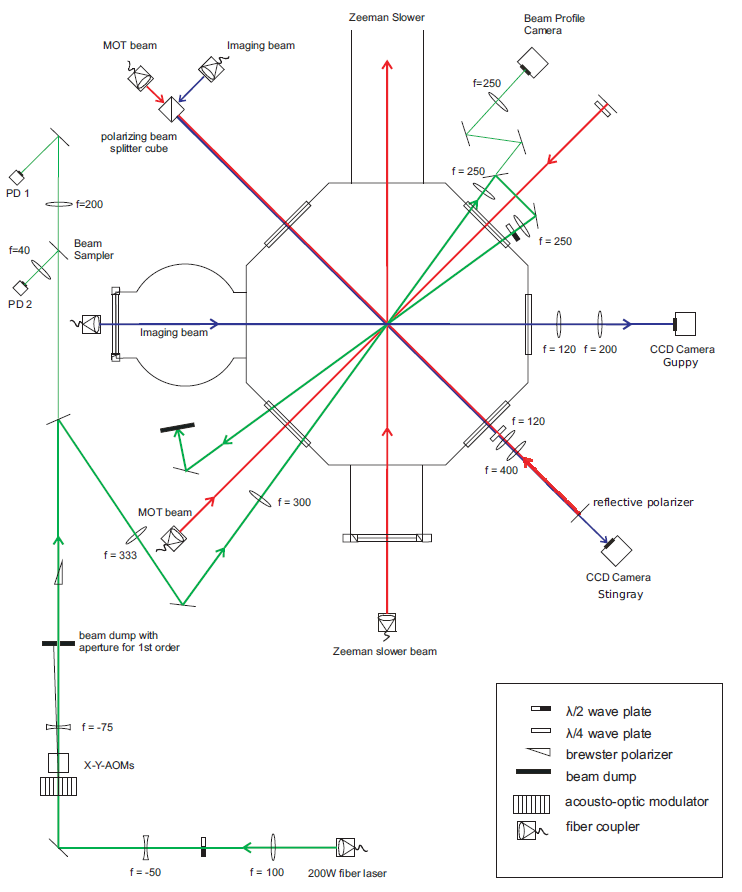
\includegraphics[width=\textwidth]{scheme}
\end{subfigure}
\caption{Scheme of the laser set-up around the vacuum chamber \cite{lompe}. The preperation of the Fermi gas uses two laser systems, consisting of the red resonant light for the \textsc{mot} and the infrared laser of the dipole trap. A second resonant laser beam is used to do absorption imaging.}
\label{scheme}
\end{figure}
\section{Imaging}

At different stages of the experiment, the atoms can be imaged by different methods. While absorption imaging is used for diagnostics, we rely on fluorescence imaging for our experiments.

\subsection{Absorption imaging}

Absorption imaging is a common method to image clouds of atoms\cite{ketterle}. A resonant beam is pointed at the sample, and partly gets absorbed. The shadow is captured on the sensor of a \textsc{ccd}-camera. It shows the density distribution along the cloud. In the classical regime, where the Fermi gas is not degenerate, a Gaussian can be fitted to this distribution to obtain the atom number. When the gas is degenerate and follows Fermi statistics, this no longer holds and the calculation gets more complicated. A detailed analysis can be found in \cite{ketterle2}.

In this setup we use a tunable, grating stabilized diode laser (Toptica \textsc{dl}-100). We take three different images. The first pictre images the atom cloud. The next picture is taken when the atom cloud is released from the trap, and the cloud is no longer visible. This image only contains the excessive imaging light wich can be subtracted from the initial image. To account for disturbances of the ambient light, a third picture is taken.

The absorption not only depends on the density but also on the scattering cross section. For resonant light, the absorption is higher and therefore we will use this technique later on to find the resonance frequency of the atoms and to determine the \textsc{ac}-Stark shift.

However, this method is not suitable for resolving single atoms, because it requires a high atomic density. One therefore has to rely on the more basic fluorescence imaging.

\subsection{Fluorescence imaging}

Our current method of imaging single photons is using the \textsc{mot} to recapture the atoms after releasing them from the deactivated microtrap \cite{timo}. The trapping light gets absorbed and the resulting fluorescence is caught on a \textsc{ccd}-camera. the amount of captured light is used to determine the atom number, which is possible with high fidelity. The current imaging setup needs long exposure times of about one second. Since all atoms are recaptured in the same \textsc{mot}, no spatial resolution is possible.

The next step will be imaging the atoms inside the microtrap, to compensate the disadvantage of the current setup. Instead of a \textsc{mot} the atoms are excited in a non-trapping optical molasse. A retro-reflected resonant laser beam intersects the dipole trap and the emitted photons are once again captured, in this setup using a high numerical aperture objective and an \textsc{emccd}-camera, that allows single photon sensitivity. By holding the atoms in the trap while imaging, the fluorescence not only allows counting the absolute number, but to see the position of the single particles.



